\documentclass[11pt,letterpaper]{article}
\usepackage[margin=0.83in,headheight=15pt]{geometry}
\usepackage[T1]{fontenc}
\usepackage{lmodern,amsmath,amssymb,mathtools,amsthm,booktabs,array,graphicx}
\usepackage{xcolor,microtype,enumitem,fancyhdr}
\definecolor{navy}{HTML}{18384E}\definecolor{teal}{HTML}{137F8C}\definecolor{pale}{HTML}{EDF4F6}
\usepackage[colorlinks=true,linkcolor=navy,urlcolor=teal,citecolor=navy]{hyperref}
\hypersetup{pdftitle={Exact scalar-radius vacuum: instability and tuned stationary branches},pdfauthor={Prepared for Christopher Michael Baird with OpenAI Codex}}
\pagestyle{fancy}\fancyhf{}
\fancyhead[L]{\small\color{navy} MQGT--SCF / EXACT COUPLED VACUUM}
\fancyhead[R]{\small 22 October 2026}
\fancyfoot[L]{\small Conditional spectral-action calculation}\fancyfoot[R]{\small\thepage}
\setlength{\parindent}{0pt}\setlength{\parskip}{5pt}
\widowpenalty=10000\clubpenalty=10000
\setlist{nosep,leftmargin=1.5em}\emergencystretch=2em
\DeclareMathOperator{\Tr}{Tr}\DeclareMathOperator{\diag}{diag}
\newcommand{\dd}{\mathrm d}\newcommand{\Lam}{\Lambda}\newcommand{\B}{\mathcal B}\newcommand{\HH}{\mathcal H}
\newtheorem{proposition}{Proposition}
\newcommand{\VacuumTable}{%
\begin{tabular}{@{}lrrrrr@{}}\toprule
Profile & $\varepsilon$ & $R$ & $h_d$ & $h_u$ & $K_{\rm rel}$\\\midrule
$f_-$ & $10^{-2}$ & 1.27816455880 & 0.209127351 & 0.194386174 & 11.64087475\\
$f_+$ & $10^{-2}$ & 1.27816454377 & 0.209126930 & 0.194385783 & 11.64069732\\
$f_-$ & $10^{-4}$ & 1.27846931626 & 0.020860089 & 0.019392704 & 11.70127067\\
$f_+$ & $10^{-4}$ & 1.27846931716 & 0.020856518 & 0.019389384 & 11.70109309\\
\bottomrule\end{tabular}}
\newcommand{\StabilityTable}{%
\begin{tabular}{@{}lrr@{}}\toprule
Quantity in the stated coordinates & $\varepsilon=10^{-2}$ & $\varepsilon=10^{-4}$\\\midrule
Smallest radial/amplitude eigenvalue & $1.86539\times10^{-2}$ & $1.87517\times10^{-4}$\\
Second radial/amplitude eigenvalue & $4.24479\times10^{-2}$ & $4.26782\times10^{-4}$\\
Largest radial/amplitude eigenvalue & $1.16560\times10^{1}$ & $1.17170\times10^{1}$\\
Charged eigenvalue (twice) & $1.59283\times10^{-2}$ & $1.60175\times10^{-4}$\\
Smallest scalar kinetic eigenvalue & $4.36350\times10^{-2}$ & $4.42349\times10^{-2}$\\
Smallest neutral kinetic eigenvalue & $1.97961\times10^{-1}$ & $1.99529\times10^{-1}$\\
\bottomrule\end{tabular}}
\newcommand{\DifferenceTable}{%
\begin{tabular}{@{}lrr@{}}\toprule
Difference $f_+-f_-$ & $\varepsilon=10^{-2}$ & $\varepsilon=10^{-4}$\\\midrule
$\Delta R$ & $-1.504\times10^{-8}$ & $8.973\times10^{-10}$\\
$\Delta h_d$ & $-4.211\times10^{-7}$ & $-3.571\times10^{-6}$\\
$\Delta h_u$ & $-3.902\times10^{-7}$ & $-3.320\times10^{-6}$\\
$\Delta c$ & $1.904\times10^{-9}$ & $1.747\times10^{-11}$\\
$\Delta(e^{-2}/\kappa)$ & $1.579\times10^{-7}$ & $1.665\times10^{-7}$\\
\bottomrule\end{tabular}}
\newcommand{\SchurLimit}{11.7018794643}
\newcommand{\EpsilonCross}{3.4178723\times10^{-8}}
\newcommand{\CheckCount}{51/51}

\begin{document}
\thispagestyle{plain}
{\small\bfseries\color{teal} BAIRD / ZORAASI RESEARCH CONTINUATION}\par
{\LARGE\bfseries\color{navy} Exact scalar--radius vacuum:\\ instability and tuned stationary branches}\par
{\large Full finite-background mode sums and the limits of restricted stability}\par
\textbf{Prepared for Christopher Michael Baird with OpenAI Codex}\hfill 22 October 2026

\colorbox{pale}{\parbox{\dimexpr\linewidth-2\fboxsep\relax}{\textbf{Result.} The untuned exact action does not stabilize the inherited common vacuum: its zero-Higgs stationary point is a scalar saddle, and a controlled large-radius limit exhibits an unbounded direction at fixed inherited subtraction. A finite numerical search finds no alternative nonzero-scalar stationary solution in the tested region, without excluding metastable extrema elsewhere. With an explicitly chosen positive scalar-mass counterterm, the exact coupled flat equations have small-field branches with positive retained radius/scalar and charged curvature. Their radius shifts are negative, opposite to the local scalar approximation. These are local minima of a restricted potential modulo exact flat directions, not a demonstration of full compactification stability or a derivation of the measured fine-structure constant.}}

\section{Question and inherited inputs}

The preceding note \cite{exact} computed scalar coefficients and the neutral response from a specified microscopic Yukawa insertion. Its scalar potential was expanded through fourth order and the radius was prescribed. We now evaluate the finite-background spectral trace itself and solve coupled scalar/radius equations. We retain the monopole matrices, four copied fermion blocks, unit dimensionless Yukawas and ten-exponential profile pair. The pinned source commit is \texttt{12fa25f}; the unchanged profile input retains its original 95 decimal digits.

The background family consists of a round sphere with $R=\Lam r$, a fixed equivariant monopole connection and two lowest scalar harmonics. Neutral amplitudes are real $h_d,h_u$, with $h_i=H_i/(\Lam R)$. All powers of these amplitudes are retained in the potential. Higher scalar harmonics, nonspherical metric modes and their tadpoles are not included. Exact fermion mode sums do not make this a complete bosonic truncation. We distinguish untuned stationarity, static local stability after a declared mass tuning, and the additional conditions for a physical vacuum.

\section{Finite-background action and flat equations}

For $f(z)=\sum_a w_a e^{-az}$, $w_a>0$, the internal Hermitian operators are
\begin{equation}
 \B_q=D_{2\oplus1\oplus1}/R+h_dS_d+h_uS_u,\quad
 \B_\ell=D_{2\oplus1}/R+h_dS_\ell,\quad \B_0=D_0/R.
\end{equation}
The matrices $S=\Gamma\mathcal M/h$ are those of \cite{exact}; the quark down and conjugate-up maps use opposite $j=1/2$ magnetic components. External momentum integration gives
\begin{equation}
 P(R,h_d,h_u)=\sum_a\frac{w_a}{a^2}
 [6\Tr e^{-a\B_q^2}+2\Tr e^{-a\B_\ell^2}+6\Tr e^{-a\B_0^2}].
 \label{eq:P}
\end{equation}
The factors include four copied blocks, colour and the full-Dirac factor $1/2$. At zero scalar background this is exactly the inherited radius trace,
\begin{gather}
 P(R,0,0)=\sum_a\frac{w_a}{a^2}(12\widehat h_0+28\widehat h_1+16\widehat h_2)(a/R^2),\qquad
 \widehat h_n(u)=\frac n2+\sum_{l\ge1}(2l+n)e^{-ul(l+n)}.
\end{gather}
No additional unbroken contribution from the scalar-coupled fermions is added.

Define the dimensionless potential
\begin{equation}
 W=\frac{4\pi^2V}{\kappa\Lam^4}=P+\alpha R^2(16h_d^2+12h_u^2)-cR^2.
 \label{eq:W}
\end{equation}
The inherited untuned case is $\alpha=0$. The optional $\alpha>0$ term is a new specified scalar-mass operator, not part of the spectral trace. It has the sphere-volume dependence of a six-dimensional scalar mass term. In the predecessor's local convention, $\alpha=m_1\delta^2/(4\pi)$.

A flat stationary solution obeys $W=W_R=W_d=W_u=0$. Eliminating the parameter $c$ gives
\begin{align}
 P_d+32\alpha R^2h_d&=0,&P_u+24\alpha R^2h_u&=0,\\
 F:=RP_R-2P&=0,&c&=P/R^2+\alpha(16h_d^2+12h_u^2).
 \label{eq:flat}
\end{align}
The counterterm cancels from $F$ at fixed $h$, but it changes the amplitudes entering that equation. Changing from $h_i$ to the radius-dependent original fields $H_i$ adds terms proportional to scalar gradients to the radius equation; stationary solutions therefore agree.

The subtraction $c$ is a coupling. Equation~\eqref{eq:flat} selects it after solving the other equations; it is not an equation of motion for another field. Holding $c=c_*$ instead gives tuned restricted stationary points with nonzero $W$. These diagnostics are recorded, but they are not flat vacua, and we do not solve for their external spacetime curvature.

\section{Analytic derivatives and static stability}

Put $g(b)=\sum_a w_a a^{-2}e^{-ab^2}$. Its derivatives are
\begin{equation}
 g'(b)=-2b\sum_a\frac{w_a}{a}e^{-ab^2},\qquad
 g''(b)=\sum_aw_a(4b^2-2/a)e^{-ab^2}.
\end{equation}
In an eigenbasis of $\B$, write $B_A=\partial_A\B$ and $B_{AB}=\partial_A\partial_B\B$. For each trace,
\begin{align}
 \partial_A\Tr g(\B)&=\sum_i g'(b_i)(B_A)_{ii},\\
 \partial_A\partial_B\Tr g(\B)
 &=\sum_{ij}g'^{[1]}(b_i,b_j)(B_A)_{ij}(B_B)_{ji}
   +\sum_i g'(b_i)(B_{AB})_{ii},\\
 g'^{[1]}(x,y)&=\frac{g'(x)-g'(y)}{x-y},\qquad g'^{[1]}(x,x)=g''(x).
 \label{eq:derivatives}
\end{align}
The only nonzero second operator derivative in $(R,h_d,h_u)$ is $B_{RR}=2D/R^3$. Nearly degenerate eigenvalues use the continuous divided-difference limit. A matrix-exponential evaluation and finite differences check these formulas independently.

At a flat solution the retained Hessian and scalar-relaxed radial curvature are
\begin{align}
 \HH_{AB}&=\partial_A\partial_B[P+\alpha R^2(16h_d^2+12h_u^2)]-2c\delta_{AR}\delta_{BR},\\
 K_{\rm rel}&=\HH_{RR}-\HH_{Rh}\HH_{hh}^{-1}\HH_{hR}.
 \label{eq:schur}
\end{align}
Their eigenvalues are derivatives of $W$ in specified coordinates, not canonical squared masses. At $W=\dd W=0$, a smooth positive Einstein-frame rescaling preserves the Hessian's inertia. It does not supply a radion kinetic term or certify freedom from ghosts.

\subsection{Charged and phase directions}

The retained scalar potential depends on $D=h_d^\dagger h_d$, $U=h_u^\dagger h_u$ and $P_c=|h_d^Ti\sigma_2h_u|^2$. Independent phases are absorbed into the right-flavour spaces of the potential trace. Rotate the up doublet relative to the down doublet by $\theta$, at fixed norms. Then $P_c=h_d^2h_u^2\sin^2\theta$, and
\begin{equation}
 T_\theta=\left.\frac{\dd^2W}{\dd\theta^2}\right|_0=2h_d^2h_u^2W_{P_c},\qquad
 \lambda_{\rm ch}=T_\theta\frac{h_d^2+h_u^2}{h_d^2h_u^2}.
 \label{eq:charged}
\end{equation}
There are two identical nonzero charged Cartesian Hessian eigenvalues $\lambda_{\rm ch}$. We compute $T_\theta$ using \eqref{eq:derivatives}, including $B_{\theta\theta}=-h_uS_u$, and check it with a separate dense angular-matrix assembly at finite $\theta$.

The other four scalar directions are gauge/phase zeros. With the adopted potential-free Stueckelberg axion, the scalar-plus-axion potential has five zero directions. Four are gauge directions and one physical phase remains flat. No axion potential is inserted to remove it. A stable radial/amplitude block alone would not have established these charged and phase properties.

\section{Untuned action: saddle and an analytic runaway}

The symmetric stationary point remains
\begin{equation}
 R_*=1.278472412043978650\ldots,\quad c_*=43.6889644825418325\ldots,\quad h_d=h_u=0.
\end{equation}
For $f_-$, its radial curvature is $K_f=11.7176182432$, but its neutral-amplitude Hessian entries are $-4.10218519448$ and $-3.07663889586$. All eight scalar Cartesian directions have corresponding negative quadratic curvature. Thus the point is a scalar saddle despite passing the radius-only test.

The full trace also changes the inference from the positive quartics. Figure~\ref{fig:untuned} compares it with its quartic polynomial. For $f_-$, a 360-point scan uses eight radii from $0.25$ to $3$, nine scalar norms from $0.03$ to $24$, and five neutral amplitude ratios. The common scalar dilation derivative $h_dP_d+h_uP_u$ is negative at every sampled point. Twelve bounded nonlinear searches are recorded with endpoints, residuals and termination status. They approach the symmetric boundary or stop at other bounds/nonzero residuals; no nonzero-scalar root meets the residual criterion. This is not a continuous-domain exclusion or a proof against all metastable extrema.

An analytic global-instability statement is stronger. Hold $h_d=h_u=h$ fixed and take $R\to\infty$. In the leading resummed heat trace, derivative and curvature terms are subleading in $1/R$, while the scalar mass is retained to all powers. The quark matrix has one zero eigenvalue and a pair with squared mass $h^2/(2\pi)$, since the two lowest harmonics have constant total squared norm $1/(2\pi)$. The lepton squared mass is uniformly distributed from zero to $h^2/(2\pi)$ over the sphere. The spectator remains uncoupled. Hence
\begin{align}
 \lim_{R\to\infty}P(R,h,h)/R^2&=\mathcal C_f(h),\\
 \mathcal C_f(h)&=\sum_a\frac{w_a}{a^3}\left[24+24e^{-z_a}+8\frac{1-e^{-z_a}}{z_a}\right],
 \qquad z_a=ah^2/(2\pi).
 \label{eq:weyl}
\end{align}
The fraction is one at zero: $\mathcal C_f(0)=56m_3$ and $\lim_{h\to\infty}\mathcal C_f(h)=24m_3$. These are iterated limits; the proof uses fixed finite $h$. The mass is resummed, not polynomially truncated \cite{Vassilevich,Iochum}.

\begin{samepage}
\begin{proposition}
The untuned action with the inherited fixed subtraction is unbounded below in the declared round-sphere/lowest-scalar family.
\end{proposition}
\begin{proof}
For the minus profile $m_3=0.8084092498040453$ and $\mathcal C_-(2)=37.6225487625902<c_*$. Along $h_d=h_u=2$, $W/R^2\to-6.06641571995$, and $W\to-\infty$. The plus profile satisfies the same strict inequality. More generally, $c>24m_3$ suffices, since then a finite $h$ exists with $\mathcal C_f(h)<c$.
\end{proof}
\end{samepage}

The negative direction involves the inherited subtraction, not negativity of the bare positive spectral trace. It rules out a global ground state for this fixed action, not all local minima. Finite-mode controls at $R=3,6,10$ check approach to \eqref{eq:weyl}; the asymptotic derivation establishes the unbounded direction.

\begin{figure}[ht]
\centering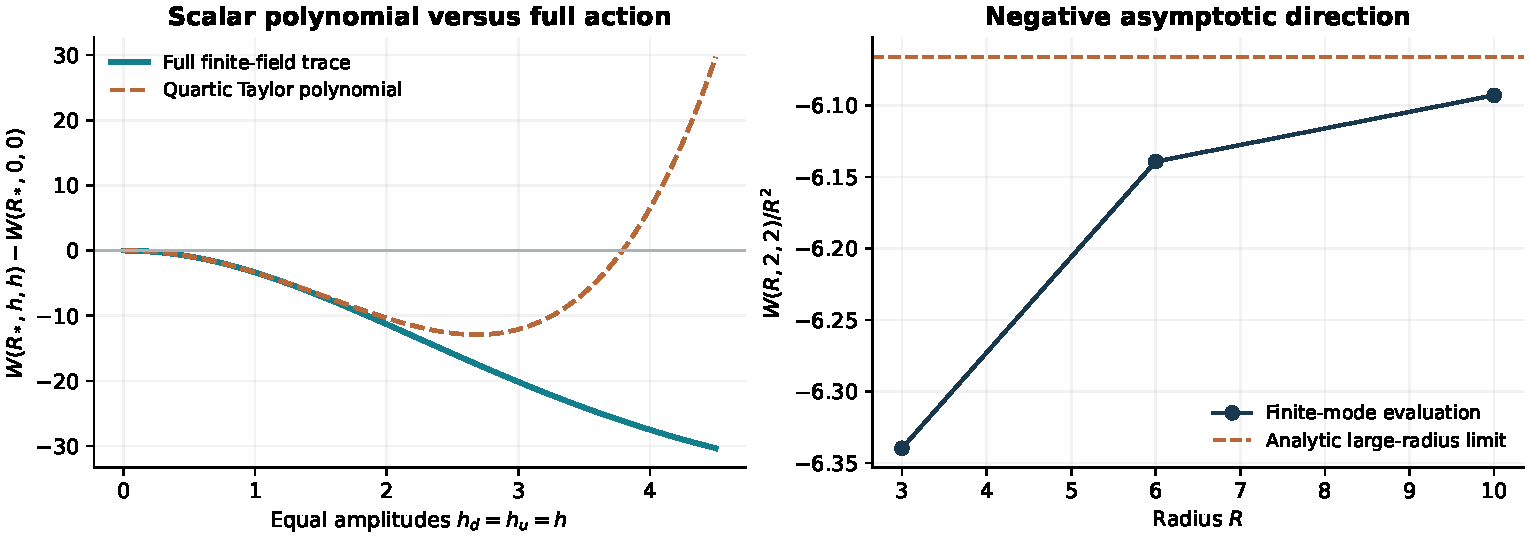
\includegraphics[width=\linewidth]{images/untuned_action.pdf}
\caption{Untuned $f_-$ action. Left: full finite-background potential at $R_*$ along $h_d=h_u$, compared with its exact-internal-mode quartic Taylor polynomial. The polynomial's upturn is absent in the full trace. Right: $W(R,2,2)/R^2$ approaches a negative analytic limit. The subtraction stays at $c_*$ throughout.}\label{fig:untuned}
\end{figure}

\section{Explicitly tuned exact stationary branches}

Choose a common scalar-mass counterterm
\begin{equation}
 \alpha(\varepsilon)=-\frac{4\pi^2A_{2,-}(R_*)}{R_*^2}
                    -\frac{2\pi^2G_-(R_*)}{R_*^2}\varepsilon.
 \label{eq:tuning}
\end{equation}
The exact $A_2,G$ of \cite{exact} then give the minus-profile symmetric-background quadratic parameter $-\varepsilon\Lam^2$. Exactly the same $\alpha$ is used for the plus profile. The critical value is $\alpha_{c,-}=0.0784300627968372$, or $\delta_c^2=1.78044971130027$ in the local counterterm convention. The local formula would have given $\delta_c^2=1.49015750336$ and cannot set the exact critical tuning.

\begin{samepage}
Solving \eqref{eq:flat} with the full trace gives:
\begin{center}\small\VacuumTable\end{center}
\end{samepage}
The scalar amplitudes are nonzero. The 12-to-16 cutoff changes of solution coordinates are below $4.6\times10^{-11}$; Hessian changes are below $4.7\times10^{-12}$. The flatness subtraction is retuned separately. For $f_-$, $c-c_*=-2.56294\times10^{-4}$ at $\varepsilon=10^{-2}$ and $-2.55455\times10^{-8}$ at $10^{-4}$. These are selected flatness adjustments, not predictions for the vacuum energy.

For comparison, holding $c=c_*$ yields restricted stationary points with $W\simeq-4.18727\times10^{-4}$ and $-4.17538\times10^{-8}$ in the two fixtures. Their nonzero potential precludes interpreting them as solutions of the flat metric equations. They are diagnostics only.

\subsection{Why the radius shift reverses sign}

Let $D=(h_d^2,h_u^2)^T$, $n=(16,12)^T$, and expand near the critical point. Exact scalar quartics give
\begin{equation}
 Q=4\pi^2\begin{pmatrix}16A_4&6C_0\\6C_0&12A_4\end{pmatrix},\quad
 b=4\pi^2n\left(A_2'-\frac{2A_2}{R_*}\right),\quad
 Q_{\rm eff}=Q-\frac{bb^T}{2K_f}.
\end{equation}
The $b$ term includes the radius dependence of the explicit counterterm at criticality. The leading branch is
\begin{equation}
 D=(2Q_{\rm eff})^{-1}2\pi^2G_-\varepsilon n+O(\varepsilon^2),\qquad
 \delta R=-b^TD/K_f+O(\varepsilon^2).
\end{equation}
The exact slope combination is $A_2'-2A_2/R_*=8.00819552\times10^{-5}>0$. The local expression is instead $-5m_1/(48\pi^3R_*)=-1.45462318\times10^{-3}$. Consequently the exact small-field branch moves to smaller radius: $\delta R=-3.07853\times10^{-4}$ and $-3.09578\times10^{-6}$ for the two minus-profile fixtures. The reversal is a finite-radius result, not a sign convention change.

The relaxed curvature tends to
\begin{equation}
 K_{\rm rel}\longrightarrow K_f-\tfrac12b^TQ^{-1}b=\SchurLimit.
\end{equation}
The exact mixing weakens the restricted curvature only slightly, versus the local predecessor's value near $7.47$. This comparison applies to the declared counterterm prescription. An unspecified radius-dependent tuning would leave both the slope and the curvature shift undetermined.

\section{Stability and profile dependence}

The minus-profile solutions have the following stability diagnostics:
\begin{center}\small\StabilityTable\end{center}
The radius/neutral-amplitude Hessian has three positive eigenvalues. Two charged eigenvalues from \eqref{eq:charged} are positive. Together with the exact symmetry zeros, these give a local minimum modulo flat directions in the retained potential. The plus profile passes the same checks. The physical axionic phase remains flat; a strict minimum is not claimed.

The finite-background two-amplitude scalar kinetic metric is computed from the heat kernels of \cite{exact},
\begin{equation}
 G_{ij}=\frac1{8\pi^2}\sum_{a,s}w_an_s\sum_{mn}
 [I_0^{mn}(S_i)_{mn}(S_j)_{nm}-aI_u^{mn}\{B,S_i\}_{mn}\{B,S_j\}_{nm}],
\end{equation}
where $I_0^{mn}=\int_0^1e^{-a[tb_m^2+(1-t)b_n^2]}\dd t$ and $I_u$ has an additional factor $t(1-t)$. This metric and the full neutral gauge kinetic matrix are positive at both fixtures. The latter includes the geometric weak response and uncoupled spectator. Neither check supplies the radion kinetic metric or all scalar/metric mixing, so it does not establish full Lorentzian stability or physical pole masses.

\subsection{The profiles no longer share a tuned vacuum}

A common $\alpha$ splits the radii and amplitudes, and flatness selection also splits $c$. The photon normalization is evaluated at each solution using the inherited null generator $N=(1,1,0)^T$, with $e^{-2}/\kappa=N^T(K/\kappa)N$:
\begin{center}\small\DifferenceTable\end{center}
These are branch diagnostics, not a determination of $\kappa$ or a measured coupling. Small differences have fewer trustworthy digits than the absolute quantities; cutoff changes and solver residuals are supplied alongside them.

Close to criticality there is a more qualitative distinction. At $R_*$, the plus-profile quadratic parameter under the same counterterm is
\begin{equation}
 m_{+,0}^2/\Lam^2=\frac{-G_-\varepsilon+2\Delta A_2}{G_+},\qquad
 \varepsilon_{\rm cross}=2\Delta A_2/G_-=\EpsilonCross.
\end{equation}
For $0<\varepsilon<\varepsilon_{\rm cross}$, the minus symmetric point is scalar-unstable while the plus symmetric point is scalar-stable. Positive $Q_{\rm eff}$ and charged quartic support a local supercritical broken branch for minus. For example, $\varepsilon=10^{-8}$ straddles the local phase boundary. This is a near-critical classification from the coefficients, not a claim of a separately resolved tiny-vev numerical root. A two-profile broken-branch comparison therefore cannot be extended uniformly to zero tuning.

\section{Validation and remaining requirements}

The package records \CheckCount{} passing checks: inherited trace and derivative normalization; matrix exponential versus eigenvalue trace; finite-difference gradient/Hessian; inherited scalar and kinetic coefficients; large-field cutoff controls; coupled-root residuals; Hessian/kinetic positivity; and a dense independent charged-orientation computation. The 360 scan points and twelve optimizer starts are diagnostics, not hundreds of independent predictions. Residuals, tolerances, search endpoints and environment versions are in \texttt{checks.json} and \texttt{results.json}.

Finite cutoffs approximate convergent spectral representations; no interval rounding enclosure or uniform infinite-tail certificate is supplied. Inputs retain 95 digits, while new matrix calculations use floating-point arithmetic. Independent numerical methods were checked in the same assistant session. There was no separate agent referee or external peer review. Compilation, PDF inspection and fresh-extraction reproduction are recorded separately at sealing.

\textbf{Established conditionally.} The untuned action has a scalar saddle and an analytic unbounded direction at fixed inherited subtraction. A specified common mass counterterm produces solved exact flat branches with positive retained static curvature transverse to symmetry directions. Exact finite-radius effects reverse the small-field radius shift, reduce the scalar-relaxation correction, and split the local symmetry-breaking threshold between the profiles.

\begin{samepage}
\textbf{Still required for a physical vacuum.} A reason for the scalar tuning and flatness subtraction; complete bosonic equations including higher-harmonic tadpoles and metric deformations; the radion/scalar kinetic metric and full fluctuation operators; a six-dimensional anomaly completion and axion potential; and independent profile/normalization selection. Global stability and lifetime of the tuned branches, physical pole masses, quantum thresholds and running remain uncomputed. These heat traces are classical spectral-action data, not a loop effective potential. The measured fine-structure constant remains unexplained.
\end{samepage}

\begin{thebibliography}{9}\small\raggedright
\bibitem{exact} C. M. Baird, prepared with OpenAI Codex, \emph{Exact internal mode sums for the scalar sector and Higgs-induced neutral kinetics}, 22 October 2026. \href{https://github.com/Cbaird26/mqgt-scf-continued/releases/tag/v2026.10.22-exact-scalar-mode-sums}{Research prerelease}; source commit \texttt{12fa25fc3f35b0ea0b65aa870a93fa0c501957d9}.
\bibitem{scalar} C. M. Baird, AI-assisted research continuation, \emph{A Microscopic Scalar and Anomaly-Complete Sector for the Shared Spectral Action}, 22 October 2026. \href{https://github.com/Cbaird26/mqgt-scf-continued/releases/tag/v2026.10.22-scalar-anomaly-sector}{Research prerelease}; commit \texttt{7cfd34114ade13d501c659492511ffbd0e32c017}.
\bibitem{Vassilevich} D. V. Vassilevich, \emph{Heat kernel expansion: user's manual}, Phys. Rep. 388 (2003), 279--360. \href{https://arxiv.org/abs/hep-th/0306138v3}{arXiv:hep-th/0306138v3}, Sec. 8.1 on mass resummation.
\bibitem{Iochum} B. Iochum, C. Levy and D. V. Vassilevich, \emph{Global and local aspects of spectral actions}, J. Phys. A 45 (2012), 374020. \href{https://arxiv.org/abs/1201.6637v1}{arXiv:1201.6637v1}.
\end{thebibliography}
\end{document}
